\documentclass[11pt, titlepage]{article}

\usepackage[a4paper, margin=1in]{geometry}
\usepackage{graphicx}
\usepackage{tabu}
\usepackage[final]{pdfpages}

\setboolean{@twoside}{false}

\author{\textbf{The Terminal}}

\title{\textbf{Coast Capital Contractor Records Database System - Requirements}}

\begin{document}

\maketitle

\tableofcontents

\clearpage

\section{Revision History}

\begin{center}
    \begin{tabular}{|| c | c | c ||}
        \hline
        Version & Description & Date \\ [0.5ex]
        \hline\hline
        1.0.0 & Initial set of requirements & 2017/07/30 \\
        \hline
    \end{tabular}
\end{center}

\section{Stakeholders}

\begin{enumerate}
    \item \textbf{Coast Capital Savings}
    \item \textbf{Jerry Jim}
    \item \textbf{Anna Scholtz}
    \item \textbf{The Terminal}
          \begin{enumerate}
            \item Vaastav Anand
            \item Anushka Agarwal
            \item Maia Mahta Kamyab
            \item Shrey Swades Nayak
            \item Stephen van Son
          \end{enumerate}
\end{enumerate}

\section{Scope}

The project scope entails building a web application to simplify data analysis and management of contractor data for Coast Capital Savings. Hiring managers are able to add and edit contracts, whereas supervisors to the hiring managers (i.e. those with admin privileges) can additionally change user permissions and manage other users. Functionalities to visualize trending data reports, filter through the contractor database, as well as automated maintenance of FX table is also within scope of the project. 

\section{Project Description}

The aim of our project is to simplify the system Coast Capital uses for capturing contractor data. Their current system requires many hours of manual data entry and complex spreadsheet manipulation, and our aim is to provide a better method of visualization, management and maintenance. The system our team (�The Terminal�) will be building will be an online web application designed for ease of use and powerful data analysis. The application aims to make it a straightforward process to add, edit, and visualize contractor data. Our application will be easy to learn for new users such that there is not a long ramp-up period for using it in comparison to using excel spreadsheets. Furthermore, since our application is an online web tool, all the contractor data within it will always be the most up to date data available so no two users are viewing different data. 

\section{Impacted Systems}

\begin{enumerate}
    \item We will be impacting the existing system that maintains the contractor records and generates expense reports based on that as our system will be completely replacing that system.
    \item We might also be impacting the current HR system as all the existing HR records might get migrated to our system in the future if the contractor system works well for Coast Capital.
    \item Our system is also likely to have an impact on Coast Capital�s budget for servers. A long term cost will be added in hosting and maintaining this system and the database. Our plan is to have it be deployed on AWS and if Coast Capital continues with that then they would have some costs associated with this after the first free year.

\end{enumerate}

\section{Impacted Groups and Individuals}

\begin{enumerate}

    \item The person who is currently in charge of maintaining contractor records and generating reports won�t have to manually add and edit the data and neither will he have to generate reports manually.
    \item The group of Hiring Managers will now be able to easily view and manipulate all contractor records.
    \item the group of Reporting Managers will be able to view contractor records who work directly under them and generate reports based on specific projects.
    \item Training other employees to generate reports and maintain the records will now be easier as the system will be user friendly.

\end{enumerate}

\section{Assumptions}

\begin{enumerate}

    \item Our system�s reporting mechanism should be very easily usable by someone who has never ever used Pivot Tables. Thus our reporting mechanism should be easy to use and very user friendly.
    \item The process of creating and modifying contractor records should be very easy to use and understand.
    \item No one except the admin should be able to delete contractor records
    \item There should be a way of recovering the data if something happens to the database.
    \item The data that will be used by our system is very sensitive data so appropriate security measures should be in place.

\end{enumerate}

\section{Dependencies}

\begin{enumerate}

    \item The main dependency of our project is on Amazon Web Services. If any of the Amazon hosting services we are using experience an outage our web application will not function properly or will not be accessible
    \item Since our team is made up of full-time university students we will not be able to work full-time on this project so the project is also dependent on our time commitment to it. 

\end{enumerate}

\section{Functional Requirements}

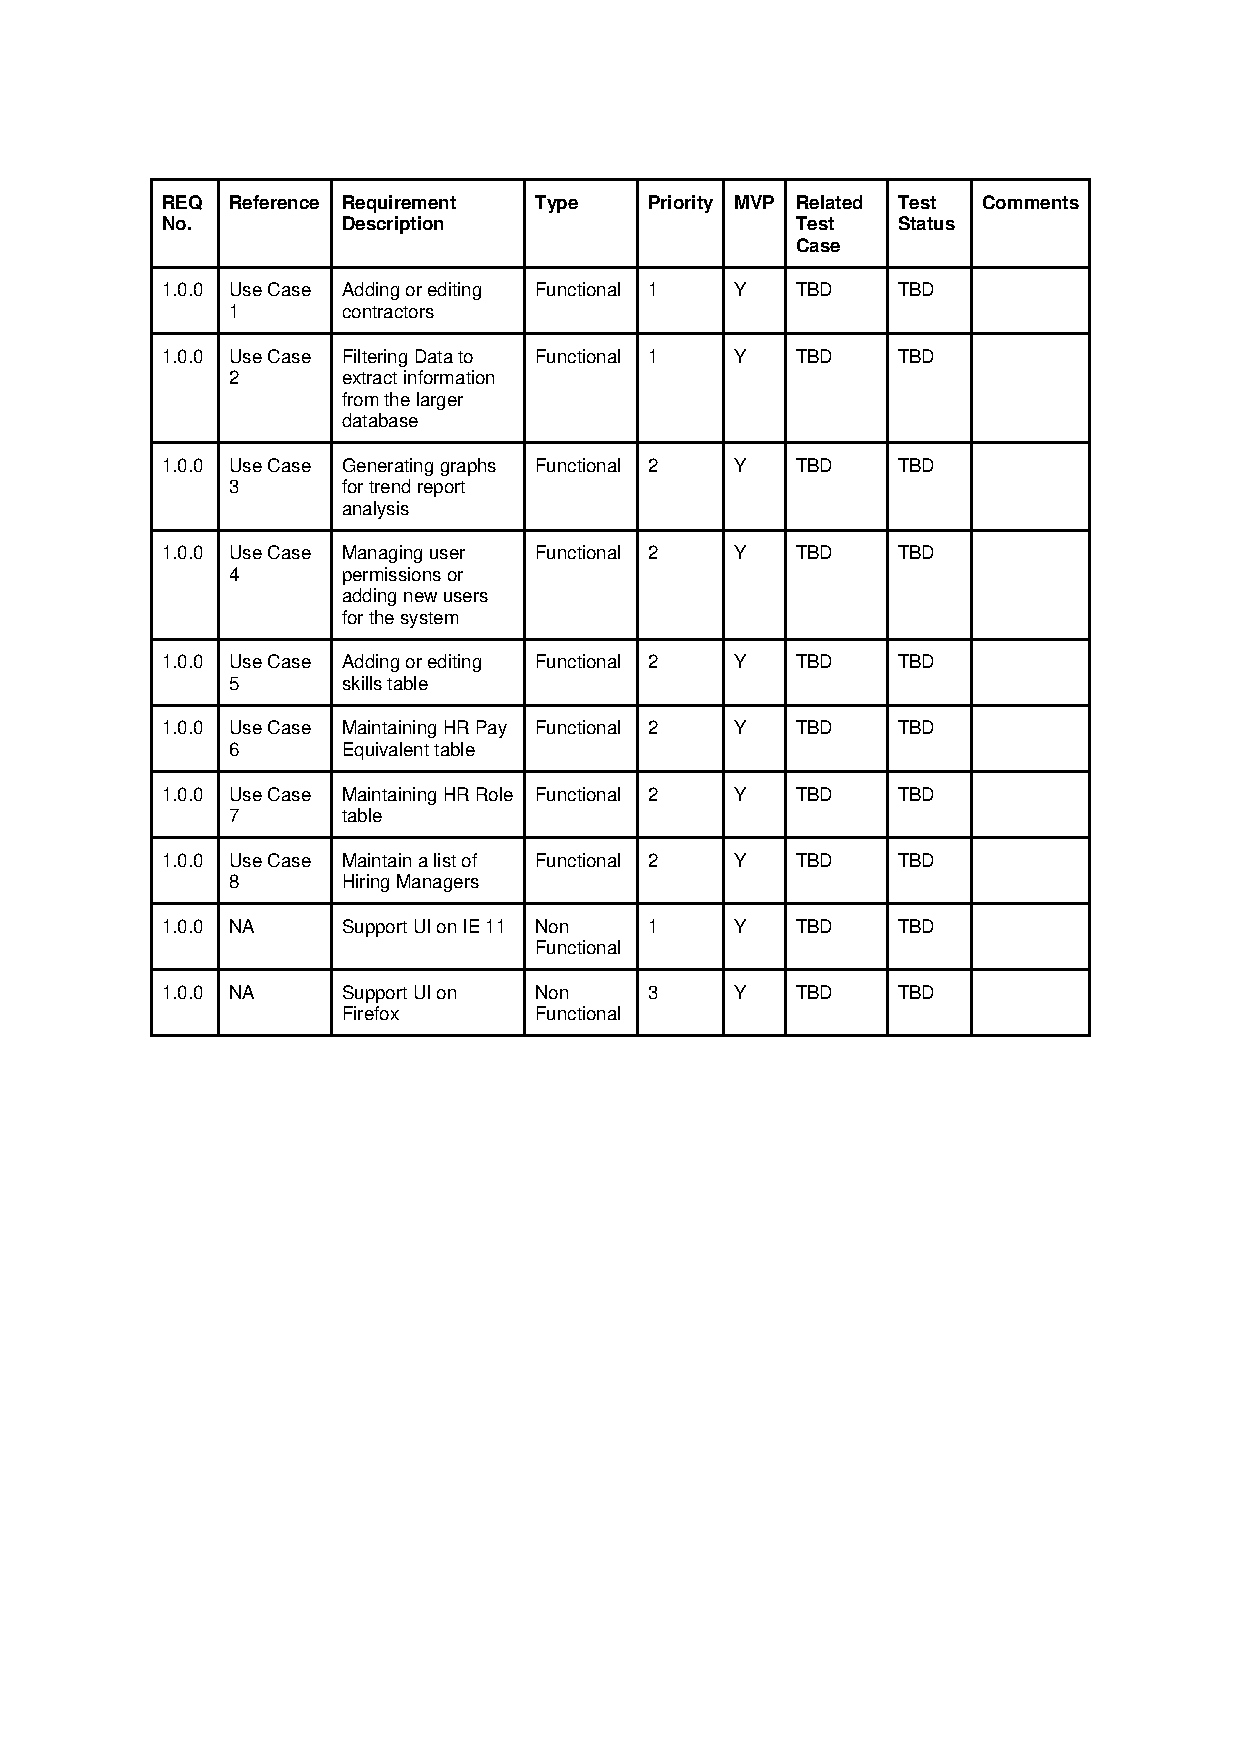
\includepdf[pages=-, pagecommand={\subsection{Requirement Traceability Matrix} \thispagestyle{empty}}, fitpaper=true]{RTM.pdf}

\subsection{Use Cases Diagram}

\subsection{Activity Flow}

\section{Non-Functional Requirements}

\subsection{Backup Needs}

\begin{enumerate}
   \item \textbf{Recoverability:} Database needs to be backed up regularly. We recommend doing either a full backup every 24 hours or a full backup every 168 hours with differentials every 24 hours. This is done so that in case if the admin indeed accidentally deletes all records or some contractor record by mistake.
   \item \textbf{Data Retention:} The data in the system is to be kept for all time, with functionality provided to toggle between inactive and active jobs.
\end{enumerate}

\subsection{Security Needs}

\begin{enumerate}
    \item \textbf{Privacy:} Sensitive information requires protection. A safety feature prompted after several minutes (2 minutes) of inactivity will result in being logged off the system. 
    \item \textbf{Accessibility:} With multiple types of users, the system must successfully hide privileged information from those who are not authorized, and also prevent lower-level users from making changes that can grant them upper-level access.
\end{enumerate}

\subsection{Capacity Needs}

\begin{enumerate}
    \item \textbf{Capability:} The system needs to be able to add and edit contractor information and visualize trending reports. The admin must be able to edit other user permissions and information.
    \item \textbf{Performance: } The system must be capable of handling a minimum expected volume of information. 
          \begin{enumerate}
            \item The system should be able to retrieve and display data in a reasonable amount of time. This is solely dependent on how much data is being transferred based on the query that was made.
            \item The system is expected to handle around 50 active contractor records per month.
          \end{enumerate}
\end{enumerate}

\subsection{Costs}

\begin{enumerate}

    \item As mentioned before, using AWS will add an extra cost for hosting the system.
    \item Additionally maintaining the database will require manpower which will have some additional costs associated with it. 

\end{enumerate}

\section{Appendix}

\subsection{Screen Mockup}

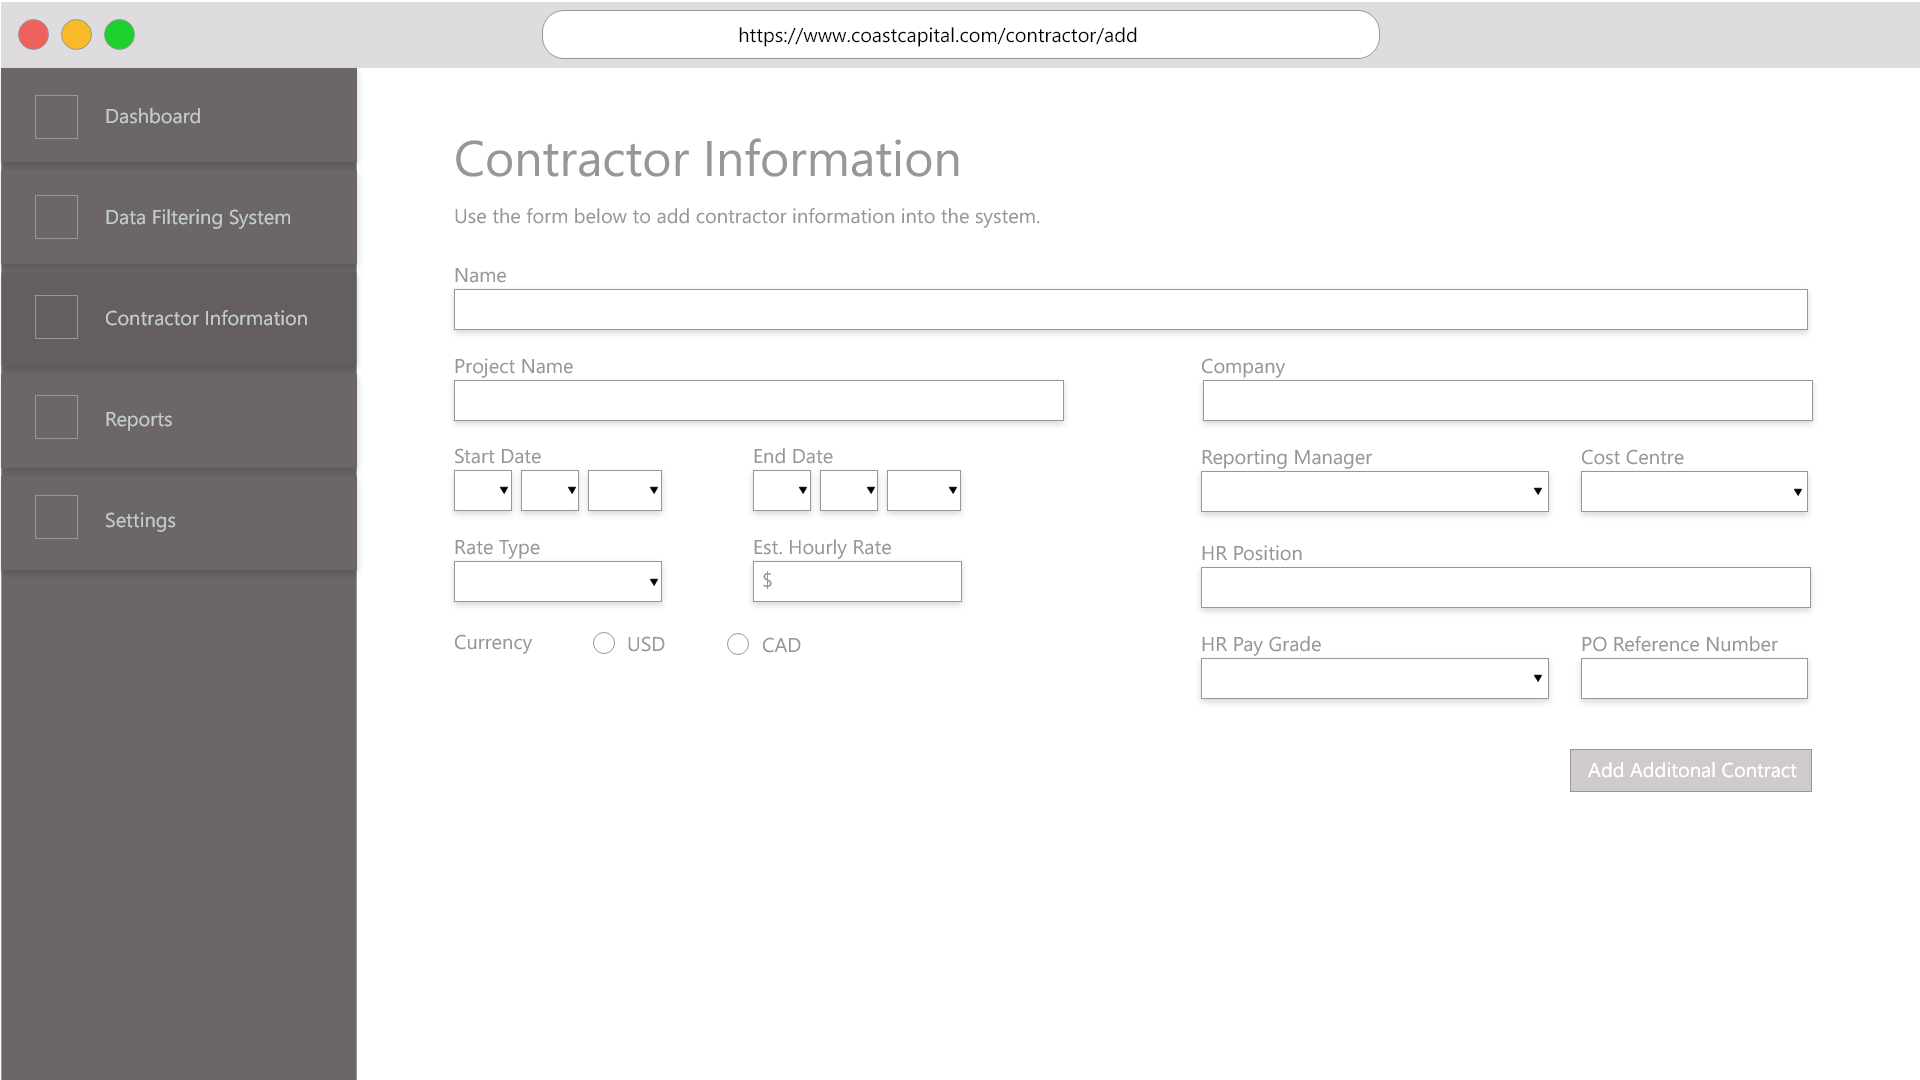
\includegraphics[width=1.0\textwidth]{../design/AddContractorUI}

The wireframe shows how a user will be able to add a contractor into the database. A simple form format provides good readability, and space is provided to add details if the contractor is assigned to multiple projects. 

\end{document}
